%
% problemstellung.tex -- Beispiel-File für die Beschreibung des Problems
%
% (c) 2020 Prof Dr Andreas Müller, Hochschule Rapperswil
%
\section{Folgerungen
\label{taylor:section:folgerungen}}
\rhead{Folgerungen}
Wie in Abbildung \ref{taylor:section:fig:FehlerRungeTaylor} ersichtlich ist, ist die Runge-Kutta Approximationen im Vergleich zur Taylor Approximation gleicher Ordnung bezüglich der logistischen Funktion genauer.
Dies gilt allerdings nur für den ausgewerteten Bereich der Gleichtung als Ganzes.
Da die Entwicklungen des Fehlers unterschiedlich verlaufen, sind beide Verfahren in gewissen Abschnitten besser.
Da man aber normalerweise die originale Funktion nicht kennt und somit auch der Fehler unbekannt ist, ziehen wir hier den defensiven Schluss und sagen, dass im Fall der logistischen Funktion die Runge-Kutte Approximation besser geeignet ist als die Taylor Approximation.

\subsection{Erklärung der Folgerung
\label{taylor:subsection:malorum}}
Wird eine Funktion nur in einem Punkt und seiner unmittelbaren Umgebung betrachtet, so kann er durch eine Funktion 1. Grades approximiert werden, bzw. einer Geraden mit der selben Steigung.
Die höheren Ordnungen spielen erst ab einem gewissen Abstand zum Auswertungspunkt eine Rolle.
Wenn wir also genug nahe bleiben, können wir eine Funktion nur durch die erste Ableitung ziemlich gut approximieren.
In diesem Fall sind die Taylor Approximation und die Runge-Kutta Approximation gleich gut, beziehungsweise die gleiche Formel.
Bei den höheren Ordnungen optimiert das Runge-Kutta Verfahren die Stelle von der es die Ableitung berechnet, indem versucht wird, einen repräsentativen Auswertungspunkt zu finden, welcher die Steigung zwischen zwei Auswertungspunkten bestmöglich trifft.
Das Taylorverfahren hingegen nimmt höhere Ableitungen dazu, welche (bei kleinen Schritten!) kaum eine Rolle spielen. 
Der Vorteil von der Taylor-Approximation ist, dass die Approximationsfunktionen wesentlich länger mit der originalen Funktion übereinstimmen \ref{taylor:section:fig:TaylorFunktion} und somit bei einer grossen Schrittweite deutlich besser sein müssen.

\begin{figure}
	\begin{center}
		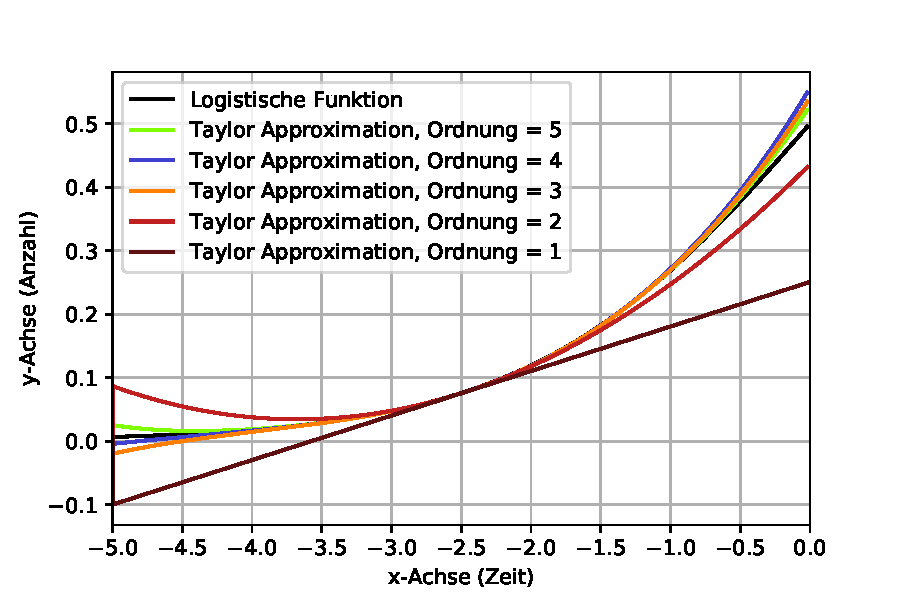
\includegraphics[width=12cm]{papers/taylor/taylorPictures/TaylorFunktion.pdf}
		\caption{Taylor Funktionen unterschiedlichen Grades im Punkt $-2.5$ als Approximation für die logistische Gleichung mit $k=1$ von $-5$ bis $-0.02$}
		\label{taylor:section:fig:TaylorFunktion}
	\end{center}
\end{figure}

